\documentclass[conference]{IEEEtran}

% *** GRAPHICS RELATED PACKAGES ***
\usepackage{graphicx}
\usepackage{pgfplots}
\usepackage{float}
\usepackage{caption}
\usepackage{subcaption}

% *** MATH PACKAGES ***
\usepackage{amsmath}
\usepackage{amssymb}
\usepackage{bm}
\usepackage{amsthm}

% *** SPECIALIZED LIST PACKAGES ***
\usepackage{algorithm}
\usepackage{algpseudocode}

% *** ALIGNMENT PACKAGES ***
\usepackage{array}

% *** PDF, URL AND HYPERLINK PACKAGES ***
\usepackage{url}

% *** TABLES PACKAGES ***
\usepackage{booktabs}
\newcommand{\ra}[1]{\renewcommand{\arraystretch}{#1}}

% *** USER DEFINITION ***
\newtheoremstyle{problemstyle} % <name>
        {3pt}                  % <space above>
        {3pt}                  % <space below>
        {\normalfont}          % <body font>
        {}                     % <indent amount}
        {\bfseries}            % <theorem head font>
        {\normalfont:}         % <punctuation after theorem head>
        {.5em}                 % <space after theorem head>
        {}                     % <theorem head spec (can be left empty, meaning `normal')>
\theoremstyle{problemstyle}

\newtheorem{Remark}{\bf Remark}

\begin{document}

\title{Data Driven Hyperparameters Optimization of One-Class Support Vector Machines for Anomaly Detection in Wireless Sensor Networks}

\author{\IEEEauthorblockN{Van Vuong~Trinh and Kim Phuc~Tran}
\IEEEauthorblockA{Division of Artificial Intelligence,\\Faculty of Information Technology,\\ Dong A University, Danang, Vietnam\\Email: vanvuong.trinh@gmail.com, phuctk@donga.edu.vn}
\and
\IEEEauthorblockN{Truong Thu Huong}
\IEEEauthorblockA{Department of Telecommunication Systems,\\School of Electronics and Telecommunications,\\Hanoi University of Science and Technology, Hanoi, Vietnam\\Email: huong.truongthu@hust.edu.vn}}

\maketitle

\begin{abstract}
One-class support vector machines (OCSVM) have been recently applied to detect anomalies in wireless sensor networks (WSNs). Typically, OCSVM is kernelized by radial bais functions (RBF, or Gausian kernel) whereas selecting hyperparameters is based upon availability of labelled anomalous, which is rarely applicable in practice. This article investigates the application of OCSVM with data-driven hyperparameters optimization. Specifically, a kernel distance based optimization criteria is used instead of labelled data based metrics such as geometric mean accuracy (g-mean) or area under the receiver operating characteristic (AUROC). The efficiency of this method is illustrated over a real data set. 
\end{abstract}

\begin{IEEEkeywords}
one-class support vector machines,  anomaly detection, wireless sensor networks, Gaussian kernel, parameters selection.
\end{IEEEkeywords}

\IEEEpeerreviewmaketitle

\section{Introduction}

\section{One-Class Support Vector Machines and Preliminaries}\label{sec:OCSVM}

In this section, we briefly recall one-class support vector machines (OCSVM) \cite{scholkopf2000support}. OCSVM is used to estimate the support of a distribution.
Notationally, let us consider a data set $\{\mathbf{x}_1,\mathbf{x}_2,\ldots,\mathbf{x}_i, \ldots,\mathbf{x}_N\}$, 
with each $\mathbf{x}_i\in \mathcal{R}^D$ belonging to a given class of interest (named target class). 
The basic idea behind the OCSVM is to separate data from the origin by finding a hyperplane with maximum margin separation from
the origin. In order to deal with nonlinearly problems, the hyperplane is defined in a high-dimensional Hilbert feature space $\mathcal{F}$ where
the samples are mapped through a nonlinear transformation $\Phi(.)$. We will work only a kernel function $k(\mathbf{x},\mathbf{y})$ instead of the scalar 
product $(\boldsymbol{\Phi}(\mathbf{x}).\boldsymbol{\Phi}(\mathbf{y}))$. To separate the data set from the 
origin, \cite{scholkopf2001estimating} solved the following quadratic program:
\begin{subequations}\label{euq:ocsvm}
\begin{align}
\underset{
	\begin{array}{c}
		 \mathbf{w}\in \mathcal{F}, \mathbf{a}, \boldsymbol{\xi} \in \mathcal{R}^N, \rho\in \mathcal{R}
	\end{array}}{\text{Minimize }} & \frac{1}{2}\left|\left| \mathbf{w}\right|\right|^2 + \frac{1}{\nu N}\sum_{i=1}^N\xi_i -\rho\\
	\label{euq:constraints}
\text{Subject to } &  (\mathbf{w}.\Phi(\mathbf{x}_i))\geq \rho -\xi_i, \quad \xi_i \ge 0 \quad \forall i=1\ldots N
\end{align}
\end{subequations}
Here, $\mathbf{w}$ is a vector perpendicular to the hyperplane in $\mathcal{F}$, and $\rho$ is the 
distance to the origin. Since the training data distribution
may contain outliers, a set of slack variables $\xi_i\geq0$ is introduced to deal with them. The
parameter $\nu \in (0,1]$ controls the tradeoff between the number
of examples of the training set mapped as positive by the
decision function
\begin{equation}
\label{equ:defosvm}
f(\mathbf{z})=\text{sgn}((\mathbf{w}.\Phi(\mathbf{x}))- \rho)
\end{equation}
and having a small value of $\left|\left| \mathbf{w}\right|\right|$ to control model complexity.\\

Using multipliers $\alpha_i,\beta_i\geq0$, \cite{scholkopf2001estimating} introduced a Lagrangian

\begin{equation}
\label{equ:lagrangian}
L(\mathbf{w}, \boldsymbol{\xi}, \boldsymbol{\alpha}, \boldsymbol{\beta},\rho)=\frac{1}{2}\left|\left| \mathbf{w}\right|\right|^2 + \frac{1}{\nu N}\sum_{i=1}^N\xi_i -\rho-\sum_{i=1}^N\alpha_i((\mathbf{w}.\Phi(\mathbf{x}_i))-\rho +\xi_i)-\sum_{i=1}^N\beta_i\xi_i.
\end{equation}
and set the derivatives with respect to the primal variables $\mathbf{w}$, $\boldsymbol{\xi}$, $\rho$ equal to zero, i.e.
\begin{eqnarray}
\label{equ:supportvm}
\frac{\partial L(\mathbf{w}, \boldsymbol{\xi}, \boldsymbol{\alpha}, \boldsymbol{\beta},\rho)}{\partial \mathbf{w}} & = 0: & \mathbf{w}=\sum_{i=1}^N\alpha_i\Phi(\mathbf{x}_i),\\%, k=1,\ldots,K, \\
\label{equ:alphai1}
\frac{\partial L(R, \mathbf{a},\boldsymbol{\xi}, \boldsymbol{\alpha}, \boldsymbol{\gamma},\rho)}{\partial \xi_i}  & =0: & \alpha_i=\frac{1}{\nu N}-\beta_i \leq \frac{1}{\nu N},  i=1,\ldots,N. \\
\label{equ:alphai2}
\frac{\partial L(R, \mathbf{a},\boldsymbol{\xi}, \boldsymbol{\alpha}, \boldsymbol{\gamma},\rho)}{\partial \rho} & = 0: & \sum_{i=1}^N\alpha_i=1\\
\end{eqnarray}

In (\ref{equ:supportvm}), all patterns $\{\mathbf{x}_i:i\in[1,\ldots,N], \alpha_i>0\}$ are called Support Vectors. From (\ref{equ:supportvm}), using the kernel function, the decision function (\ref{equ:defosvm}) is transformed into a kernel expansion 
\begin{equation}
\label{equ:defosvmker}
f(\mathbf{x})=\text{sgn}\left(\sum_{i=1}^N\alpha_i k(\mathbf{x}_i, \mathbf{x})- \rho\right)
\end{equation}
Substituting (\ref{equ:supportvm}), (\ref{equ:alphai1}) and (\ref{equ:alphai2}) into (\ref{equ:lagrangian}), and using the kernel function, we have 
\begin{equation}
\label{equ:lagrangianalpha}
L(\boldsymbol{\alpha})=-\frac{1}{2}\sum_{i=1}^N\sum_{j=1}^N \alpha_i\alpha_j k(\mathbf{x}_i, \mathbf{x}_j).
\end{equation}
Then, we obtain the dual problem
\begin{subequations}\label{euq:ocsvmker}
\begin{align}
\underset{
	\begin{array}{c}
		 \mathbf{\alpha}
	\end{array}}{\text{Minimize }} & \sum_{i=1}^N\sum_{j=1}^N \alpha_i\alpha_j k(\mathbf{x}_i, \mathbf{x}_j)\\
\text{Subject to } & 0\leq \alpha_i\leq \frac{1}{\nu N}, \quad \forall i=1\ldots N, \sum_{i=1}^N\alpha_i=1 
\end{align}
\end{subequations}
\cite{scholkopf2001estimating} shown that at the optimum, the two inequality constraints (\ref{euq:constraints}) 
became equalities if $\alpha_i$ and $\beta_i$ are nonzero, which implies $0<\alpha_i<\frac{1}{\nu N}$. Thus, the value of $\rho$
can be recovered by exploiting that for any such $\alpha_i$, the corresponding pattern $ \mathbf{x}_i$ satisfies
\begin{equation}
\label{equ:rho}
\rho=\langle\mathbf{w},\Phi(\mathbf{x}_i)\rangle=\sum_{j=1}^N\alpha_j k(\mathbf{x}_j, \mathbf{x}_i)
\end{equation}

\section{Description of Anomaly Detection Procedure for WSNs}



\section{Illustrative Example}\label{sec:Illustrative}

This section investigates the efficiency of anomaly detection algorithm over a real data set. The source code is freely available at \url{https://github.com/trinhvv/wsn-ocsvm-dfn}. All computation was performed on a platform with 2.6 GHz Intel(R) Core(TM) i7 and 16GB of RAM.

\begin{figure}[H]
\centering
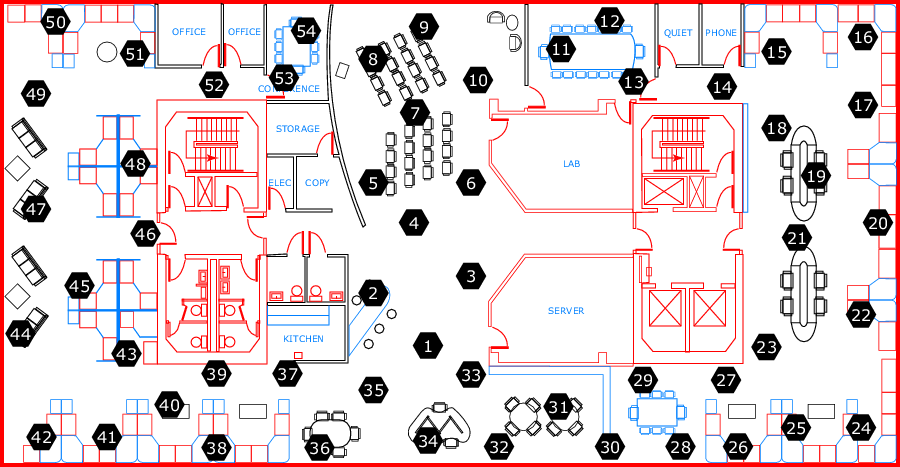
\includegraphics[scale=.25]{Figs/ibrl_wsn.png}
\caption{A map of sensors' location. (Source: \cite{Buonadonna2005})}
\label{fig:sensor_map}
\end{figure}

\begin{figure}[H]
\centering
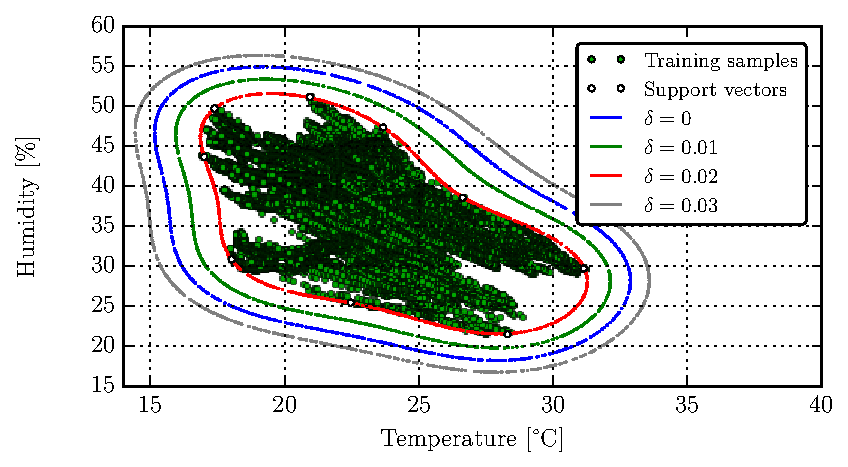
\includegraphics[scale=.6]{Python/data_description.pdf}
\caption{Discrimination boundaries with some $\delta$'s values. }
\label{fig:domain_boundary}
\end{figure}

\begin{table}[H]
\centering
\begin{tabular}{lccccccc}
\toprule
$\delta$ & 0.000 & 0.01 & 0.02 & 0.03 \\\midrule[\lightrulewidth]
DR [\%] & 100 & 100 & 100 & 100 \\
\emph{FPR} [\%] & 0 & 0 & 0 & 0 \\\bottomrule
\end{tabular}
\caption{DR and FPR versus $\delta$.}
\label{table:delta_eval}
\end{table}

\begin{figure*}
\centering
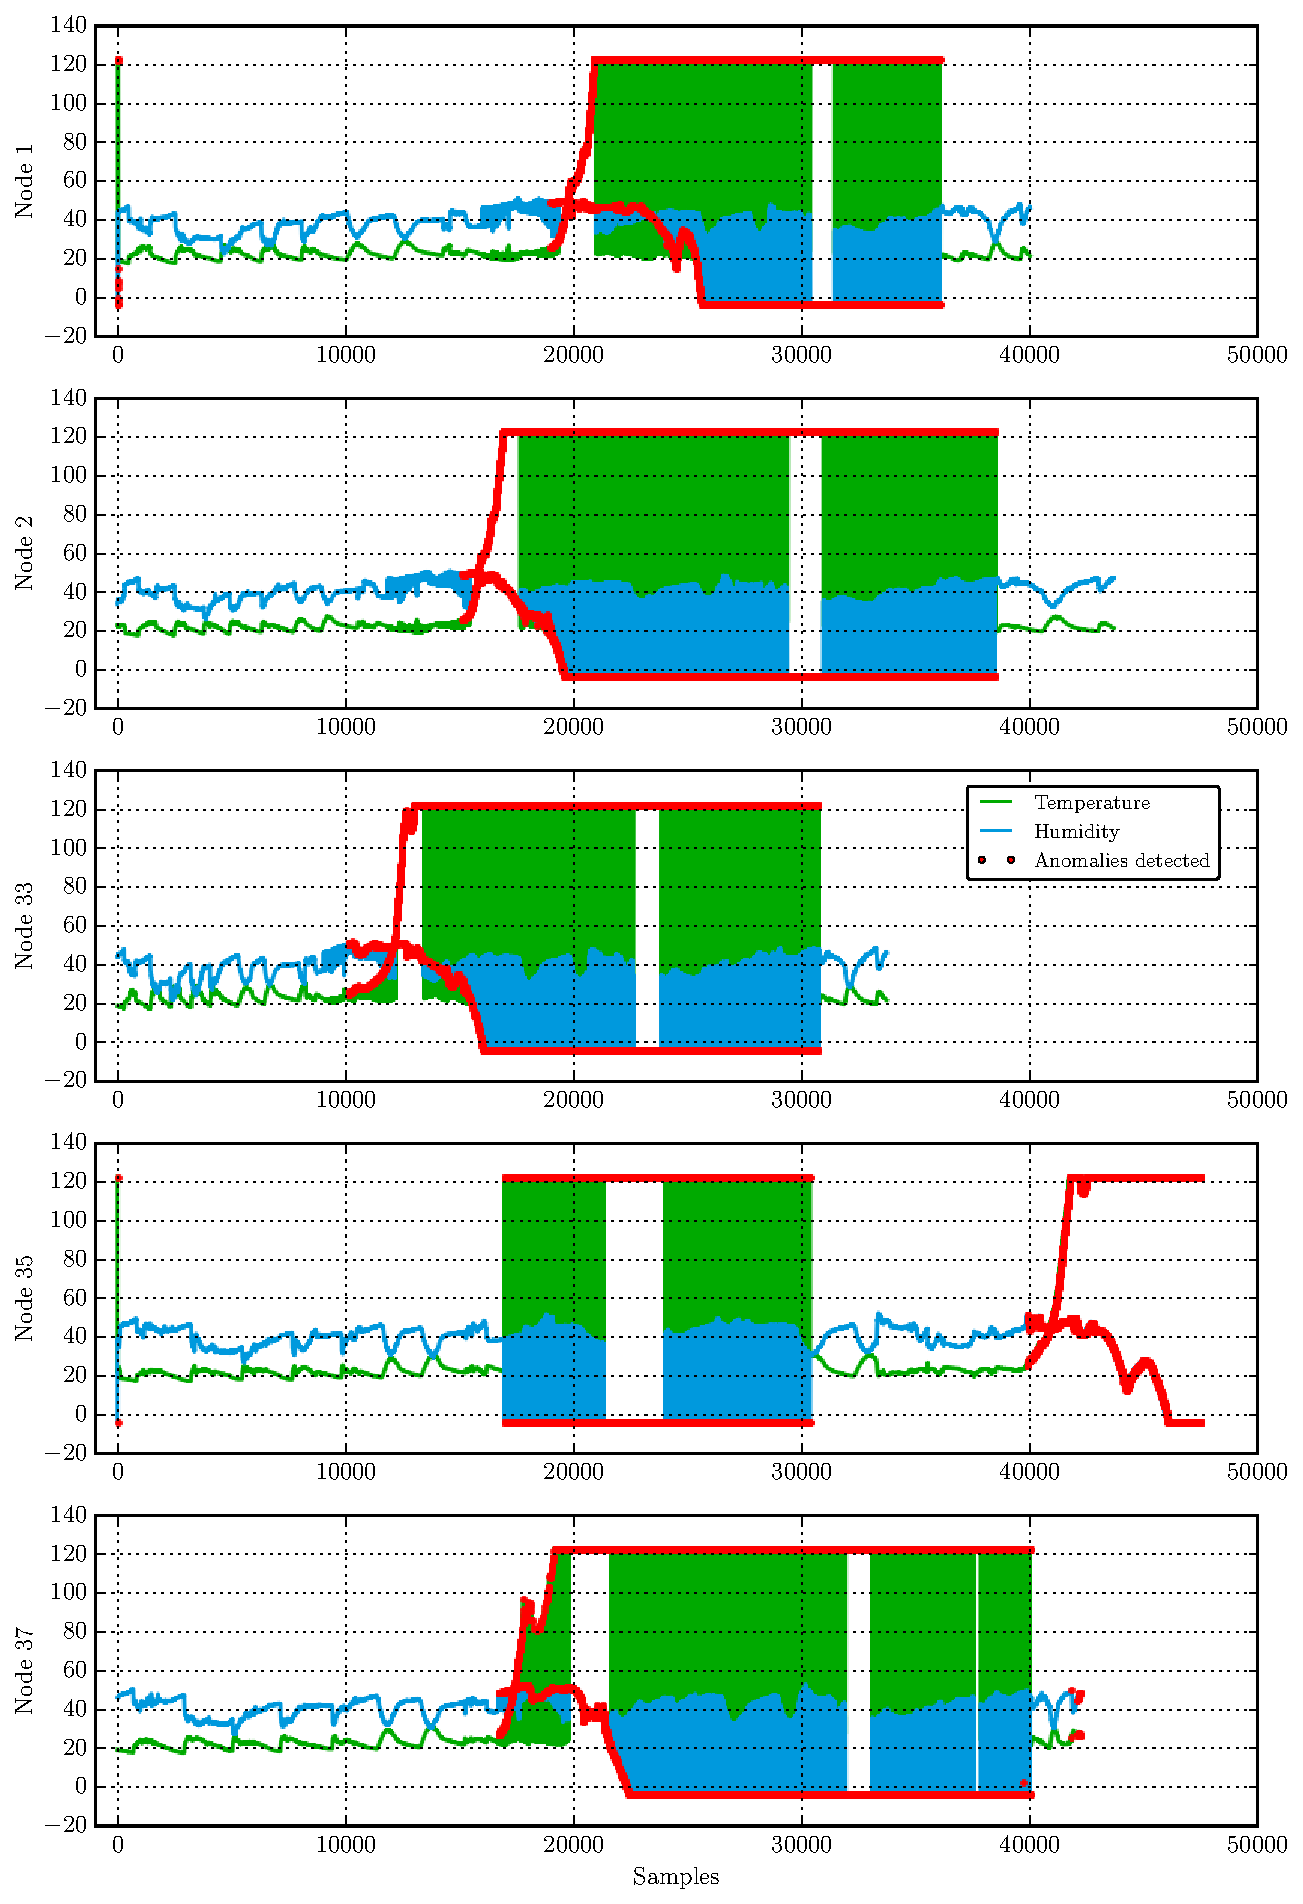
\includegraphics[scale=.7]{Python/time_validation.pdf}
\caption{Anomaly detection validation upon whole IBRL data set on $5$ nodes. Almost apparent anomalies, i.e. temperature and humidity measurements that are too high or too low, are detected.}
\label{fig:time_valid}
\end{figure*}

\bibliographystyle{IEEEtran}
\bibliography{wsnbib,svmbib,ocsvmbib,ibrlbib,miscbib}

\end{document}


